\section{Расчетно-конструкторская часть}
    \subsection{Расчет основных параметров двигателя}
        Пусковой ток
        \begin{gather*}
            I_\text{п} = 5,5 \cdot I_\text{н}.%,\\
            %I_\text{п} = 5,5 \cdot 0,76 = 4,18 \; \text{А}.
        \end{gather*}

        Номинальное скольжение
        \begin{gather*}
            S_\text{н} = \frac{n_0 - n_\text{н}}{n_0}.%,\\
            %S_\text{н} = \frac{1500 - 1350}{1500} = 0,1.
        \end{gather*}

        Критическое скольжение
        \begin{gather*}
            S_\text{кр} = S_\text{н} \cdot
                \left( \lambda_{max} + \sqrt{\lambda_{max}^2 - 1} \right).%,\\
%            S_\text{кр} = 0,1 \cdot
%                \left( 2,1 + \sqrt{2,1^2 - 1} \right) = 0,416.
        \end{gather*}

        Номинальный момент
        \begin{gather*}
            M_\text{н} = \cfrac{P_\text{н}}
                {2\pi \cdot \cfrac{n_\text{н}}{60}}.%,\\
%            M_\text{н} = \frac{120}{2\pi \cdot \cfrac{1350}{60}}
%                = 0,849 \; \text{Н} \cdot \text{м}.
        \end{gather*}

        Максимальный момент двигателя
        \begin{gather*}
            M_{max} = \lambda \cdot M_\text{н}.%,\\
%%%%%%%%            M_{max} = 2,2 \cdot 0,849 = 1,867 \; \text{Н} \cdot \text{м}.
        \end{gather*}

        Сопротивление статора
        \begin{gather*}
            R_s = \frac{\left(\cfrac{U_\text{н}}{\sqrt{3}}\right)
                \cdot (1 - S_\text{н}) \cdot 1,5}{c_1 \cdot
                    \left(1+\cfrac{c_1}{S_\text{кр}}\right) \cdot
                        M_{max} \cdot (P_\text{н} + \Delta P_\text{Т})}.%,\\
       %     R_s = \frac{\left(\cfrac{220}{\sqrt{3}}\right) \cdot (1-0,1)
       %         \cdot 1,5}{1,026 \cdot \left(
       %            1+\cfrac{1,026}{S_\text{кр}}\right) 1,867 \cdot
       %                 (120 + DP_T)} = 0,18 \; \text{Ом}
        \end{gather*}

        Сопротивление ротора
        \begin{gather*}
                R_r = \frac{P_\text{н} + \Delta P_\text{Т}}
                    {3 \cdot (1-S_\text{н}) \cdot i_\text{к}^2
                        \cdot I_\text{н}^2}.%,\\
%                R_r = \frac{P_\text{н} + \Delta P_\text{Т}}
%                    {3 \cdot (1-S_\text{н}) \cdot i_\text{к}^2
%                        \cdot I_\text{н}^2} = 0,15 \; \text{Ом}.
        \end{gather*}

        Расчет индуктивности статора
        \begin{gather*}
            L_s = \frac{\cfrac{U_\text{н}}{\sqrt{3} \cdot
                (2\pi \cdot f \cdot I_\text{н})}}{\sqrt{1 - \cos^2 f}
                    - \cos f \left(\cfrac{S_\text{н}}{S_\text{кр}}\right)}.%,\\
%            L_s = \frac{\cfrac{220}{\sqrt{3}} \cdot
%                (2\pi \cdot 50 \cdot 0,76)}{\sqrt{1 - 0,66^2}
%                    - 0,66 (0,416)} = 0,0043 \; \text{Гн}.
        \end{gather*}

        Формула рассчета индуктивность ротора
        \begin{gather*}
            L_r = L_s.%,\\
%            L_r = 0,0043 \; \text{Гн}.
        \end{gather*}

        Индуктивность намагничивания
        \begin{gather*}
            L_m = L_s - L_{1s}.
            %L_m = L_s - L_{1s} = 0,00382 \; \text{Гн}.
        \end{gather*}

        Конструктивная постоянная
        \begin{gather*}
            C_{1r} = 1+\frac{L_{1s}}{L_m}.
            %C_{1r} = 1+\frac{L_{1s}}{L_m} = 0,0109.
        \end{gather*}

        Вычислим время разгона
        \begin{gather*}
            t_\text{р} = \frac{\omega_\text{н}}{
                \cfrac{M_\text{н}}{j}}.
%            t_\text{р} = \frac{\omega_\text{н}}{
%                \cfrac{M_\text{н}}{j}} = 0,13 \; \text{с}.
        \end{gather*}

        Номинальная угловуя скорость
        \begin{gather*}
            \omega_\text{н} = \frac{2\pi n_\text{н}}{60}.
%            \omega_\text{н} = \frac{2\pi n_\text{н}}{60} 
%                = \frac{2 \cdot 3,14 \cdot 1350}{60} = 141 \; \text{мин}^{-1}.
        \end{gather*}

        Скорость идеального холостого хода
        \begin{gather*}
            \omega_0 = \frac{2\pi n_0}{60}.
%            \omega_0 = \frac{2\pi n_0}{60} 
%                = \frac{2 \cdot 3,14 \cdot 1500}{60} = 157 \; \text{мин}^{-1}.
        \end{gather*}

        Индуктивное сопротивение статора
        \begin{gather*}
            X_s = 2\pi \cdot 50 \cdot L_s.
%            X_s = 2\pi \cdot 50 \cdot L_s
%                = 6,28 \cdot 50 \cdot 0,0043 = 1,35 \text{Ом}.
        \end{gather*}
        
        Индуктивное сопротивление ротора
        \begin{gather*}
            X_r = 2\pi \cdot 50 \cdot L_r.
%            X_r = 2\pi \cdot 50 \cdot L_r
%                = 6,28 \cdot 50 \cdot 0,0043 = 1,35 \text{Ом}.
        \end{gather*}

        \begin{figure}[h!]
            \center{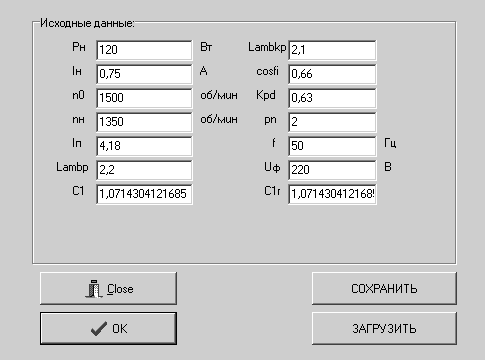
\includegraphics[width=0.6\linewidth]{img/static-scr2}}
            \caption{Входные данные для расчета параметров электродвигателя}
            \label{fig:static-scr2}
        \end{figure}       

        Для рассчета параметров двигателя и построения механических характеристик воспользуемся программой STATIC. 
        На рисунке \ref{fig:static-scr2} изображено окно программы со входными данными для рассчета.

        Рассчитанные параметры электродвигателя, а также построенные
        механические характеристики показаны на рисунке \ref{fig:static-scr1}.
        Блее детальный вид характеристики, построенной используя однофазную
        схему замещения, приведен на рисунке \ref{fig:motor-mh1}.  А
        механическая характеристика, рассчитанная по формуле Клосса, изображена
        на рисунке \ref{fig:motor-mh2}.

        \begin{figure}[h!]
            \center{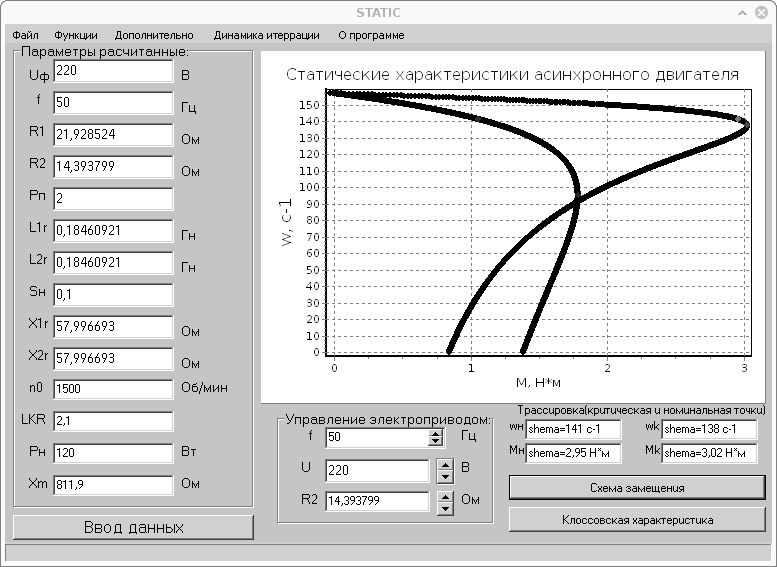
\includegraphics[width=1.0\linewidth]{img/static-scr1}}
            \caption{Окно результатов расчета параметров двигателя}
            \label{fig:static-scr1}
        \end{figure}

        \begin{figure}[h!]
            \center{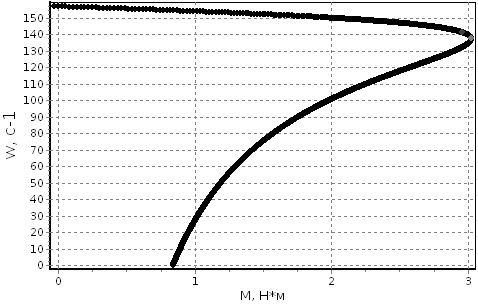
\includegraphics[width=0.6\linewidth]{img/motor-mh1}}
            \caption{Механическая характеристика двигателя, построенная по схеме замещения}
            \label{fig:motor-mh1}
        \end{figure}

        \begin{figure}[h!]
            \center{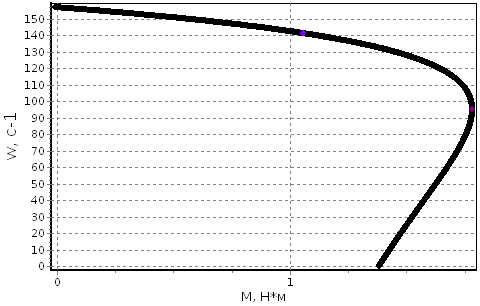
\includegraphics[width=0.6\linewidth]{img/motor-mh2}}
            \caption{Механическая характеристика двигателя, построенная по формуле Клосса}
            \label{fig:motor-mh2}
        \end{figure}

    \subsection{Моделирование системы скалярного управления асинхронного
        электропривода с к. з. ротором}

        Асинхронный привод со скалярным частотным управлением используется для
        механизмов средней и малой мощности, который не требуют глубокого
        регулирования скорости и высокого качества переходных процессов.

        Уравнение электромагнитных контуров АД в установившемся режиме будет
        иметь вид
        \begin{gather*}
            \left\{
            \begin{aligned}
                \frac{\tilde U_s}{\omega_s} =\tilde I_s\frac{Rs}{\omega_s}+
                    j\tilde \Psi_s=\tilde I_s\frac{R_s}{\omega_s}+
                        jL_{s\sigma}\tilde I_s +j\tilde \Psi_m\\
                0 = \tilde I_r\frac{R_r}{\beta}+j\tilde \Psi_r =
                    \tilde I_r\frac{R_r}{\beta}+jL_{r\sigma}\tilde I_r+
                        j \tilde \Psi_m,\\
            \end{aligned}
            \right.
        \end{gather*}

        где $\beta = \omega_s - \omega_r = S\omega_s$ -- абсолютное скольжение АД;\par
        $\tilde \Psi_m = L_m \tilde I_m = L_m(\tilde I_s + \tilde I_r)$ -- потокосцепление
        в воздушном зазоре.

        Приведенной системе уравнений соответствует эквивалентная схема
        замещения, которая представлена на рисунке \ref{fig:ad-zam}.  

        \begin{figure}[h!]
            \center{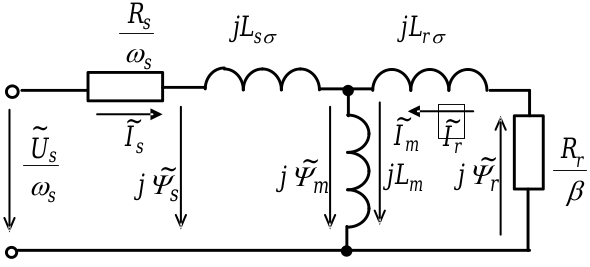
\includegraphics[width=0.6\linewidth]{img/ad-zam}}
            \caption{Эквивалентная схема замещения асинхронного двигателя с к. з. ротором}
            \label{fig:ad-zam}
        \end{figure}

        Передаточная функция регулятора напряжения внешнего контура в виде
        \begin{gather*}
            W_{PUs}(p)=\frac{\pi}{2\sqrt{3}}\cdot\frac{k_{Id}}{k_{Us}R_D} \cdot
                \frac{(T_D + T_F) p+1}{T_{H2}p},
        \end{gather*}

        где $k_v$ -- коэффициент усиления КВ.

        \begin{gather*}
            R_D = \frac{\pi^2}{18} \cdot \frac{L_s}{T_r(1 - \sigma)S_1},
        \end{gather*}

        где $T_D=R_D C_F$ -- эквивалентное сопротивление и эквивалентная
        постоянная времени объекта <<АИН -- АД>>;\par
        $S_1$ -- расчетный параметр,
        который косвенно отображает желаемую жесткость механических
        характеристик ЭП (для расчетов можно принять равным 0,1);\par
        $k_{Ui}$ -- коэффициент передачи датчика напряжения на входе АИН; 
        $T_H = k_{kUi}Tv$ --квивалентная постоянная времени интегрирования
            регулятора напряжения на входе АИН;\par
        $k_{kUi}$ -- аладочный коэффициент, значения которого превышают 1. 

        С помощью ПЧ может быть реализована нужная зависимость напряжения
        статора АД от частоты. Закон частотного регулирования, который
        реализованный в ПЧ должен выполняться при $U_S \leq U_{SH}$ для
        предотвращения питания АД увеличенным напряжением. При необходимости
        дальнейшего повышения частоты вращения напряжение статора АД должно
        быть ограничено, а регулирование скорости в этой зоне осуществляется
        лишь за счет повышения частоты.
        \begin{gather*}
            \left\{
            \begin{aligned}
                \frac{d\Phi_{sx}}{dt} = U_{sx} - R_s i_{sx} + \omega_k \Psi_{sy}\\
                \frac{d\Phi_{sy}}{dt} = U_{sy} - R_s i_{sy} + \omega_k \Psi_{sx}\\
                \frac{d\Phi_{rx}}{dt} = R_s i_{sx} + (\omega_k-\omega) \Psi_{ry}\\
                \frac{d\Phi_{ry}}{dt} = R_s i_{sy} + (\omega_k-\omega) \Psi_{rx},\\
            \end{aligned}
            \right.
        \end{gather*}

        где $\Psi_{sx}, \Psi_{sy}$ -- потокосцепления эквивалентных статорных
            контуров;\par
        $\Psi_{rx}, \Psi_{ry}$ -- потокосцепления эквивалентных роторных
            контуров;\par
        $i_{sx}, i_{sy}$ -- эквивалентные  токи статора;\par
        $i_{rx}, i_{ry}$ -- эквивалентные  токи ротора;\par
        $R_s, R_r$ -- активные сопротивления фазных обмоток статора и ротора.

        Для решения этой системы уравнений ее необходимо дополнить уравнениями
        связи эквивалентных токов и потокосцеплений машины. В системе координат
        (х–у) эквивалентные потокосцепления и токи статора и ротора двигателя
        связаны друг с другом следующими уравнениями
        \begin{gather*}
            \left\{
            \begin{aligned}
                \Psi_{sx} = L_s i_{sx} + L_m i_{rx}\\
                \Psi_{sy} = L_s i_{sy} + L_m i_{rx}\\
                \Psi_{rx} = L_s i_{sx} + L_r i_{rx}\\
                \Psi_{ry} = L_s i_{sy} + L_r i_{rx}\\
            \end{aligned}
            \right.
        \end{gather*}

    \subsection{Математическое описание и динамическая модель АД как обобщенной
        электрической машины}

        Структурная схема модели в фазных координатах получается весьма сложной
        из-за наличия переменных коэффициентов в уравнениях связи фазных токов
        и потокосцеплений машины, зависящих от мгновенного значения угла
        поворота ротора относительно магнитных осей статора двигателя. С целью
        упрощения математических моделей систему уравнений трехфазной
        асинхронной машины, записанную в фазных координатах, принято
        представлять в ортогональной системе координат (х–у), вращающейся в
        пространстве в общем случае с произвольной угловой скоростью $\omega_k$.

        Эквивалентные напряжения статора в системе координат (х–у) связаны с
        фазными напряжения трехфазной машины следующими соотношениями
        \begin{gather*}
            U_{sx} = \frac{2}{3} \left[ U_\text{ФА}\cos\omega_k t+U_\text{ФВ}
                \cos\left(\omega_k t-\frac{2\pi}{3}\right)+U_\text{ФС} \cos
                    \left( \omega_k t+\frac{2\pi}{3}\right)\right],\\
            U_{sy} = -\frac{2}{3} \left[ U_\text{ФА}\cos\omega_k t+U_\text{ФВ}
                \cos\left(\omega_k t-\frac{2\pi}{3}\right)+U_\text{ФС} \cos
                    \left( \omega_k t+\frac{2\pi}{3}\right)\right],\\
        \end{gather*}

        Аналогичные соотношения связывают эквивалентные значения токов и
        потокосцеплений двигателя с соответствующими фазными значениями
        переменных. Подставляя в эти уравнения выражения для реальных фазных
        напряжений
        \begin{gather*}
            U_\text{ФА} = U_m\cos(\omega_0 t + \varphi_0),\\
            U_\text{ФВ} = U_m\cos\left(\omega_0t-\frac{2\pi}{3}+\varphi_0\right),\\
            U_\text{ФC} = U_m\cos\left(\omega_0t+\frac{2\pi}{3}+\varphi_0\right),\\
        \end{gather*}

        Можно получить выражения для составляющих напряжений в эквивалентной
        2-хфазной системе координат
        \begin{gather*}
            U_{sx} = U_m \cos [(\omega_0 - \omega_k)t + \varphi_0],\\
            U_{sy} = U_m \sin [(\omega_0 - \omega_k)t + \varphi_0],\\
        \end{gather*}

        где $U_m$ -- амплитудное значение фазного напряжения;
        $\omega_0$ -- частота вращения поля статора двигателя в пространстве;
        $\varphi_0$ -- начальная фаза напряжения фазы А.

        Система уравнений электромагнитного равновесия асинхронного двигателя в форме Коши в системе координат (х–у) может быть представлена следующим образом

    \subsection{Разработка аппаратной части системы управления автономным
        инвертором напряжения}

%        Разработанная система управления построена на основе отладочного модуля
%        микроконтроллеров серии STM32F100х фирмы ST Microelectronics.

        Блок управления автономным инвертором напряжения реализует
        модулирование ШИМ сигнала управления трехфазным мостом синусоидальным
        сигналом переменной частоты и амплитуды. Амплитуда и частота
        синусоидального сигнала изменяются в соответствии со скалярным законом
        регулирования частоты вращения ротора асинхронного двигателя с
        постоянством отношения $U/f$.

        Принципиальная электрическая схема системы управления АИН представленна
        на рисунке \ref{fig:control-schematic}.

        \begin{sidewaysfigure}
            \center{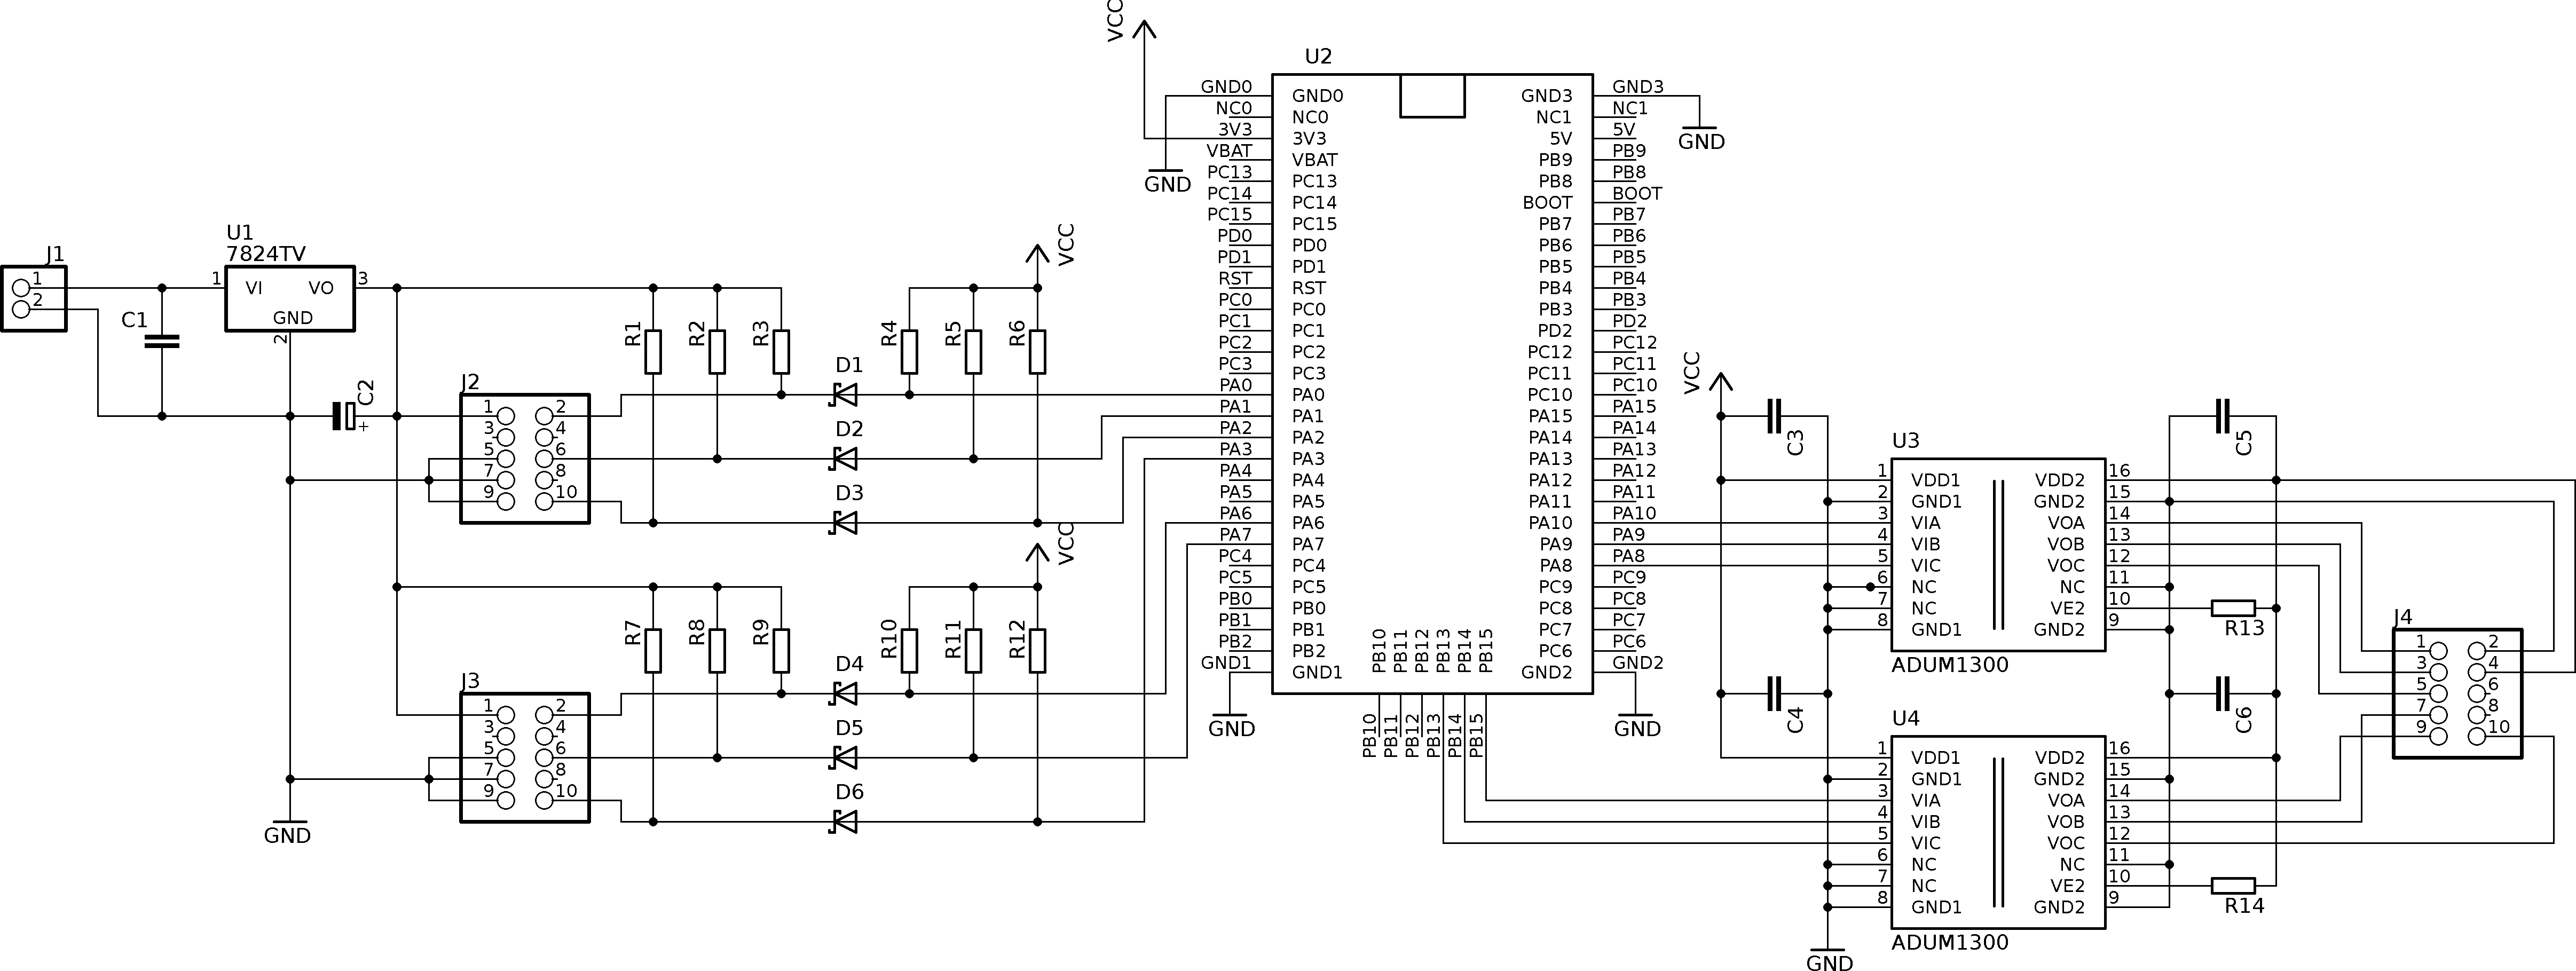
\includegraphics[width=1.0\linewidth]{img/control-schematic}}
            \caption{Принципиальная электрическая схема блока управления АИН}
            \label{fig:control-schematic}
        \end{sidewaysfigure}

        Сигнал управления трехфазным мостом силовых транзисторов АИН снимается
        с выводов PA8, PA9, PA10 (верхние транзизторы моста; фаза A, B и C
        соответственно) и PB13, PB14, PB15 (фаза A, B и C; нижние транзисторы).
        Далее сигнал подается на схему гальванической развязки выполненную на
        двух микросхемах U3 и U4. 
        
        Гальваническая развязка силового блока и блока управления необходима
        так как потенциал общего провода силовой части электропривода может
        иметь значение напряжения питающей сети. Поэтому применением цифровх
        изоляторов с напряжением пробоя болле 2 КВ, обеспечивается защита
        оператора установки от поражения электрическим током, а так же
        буферизация и защита модуля управления от аватийных ситуаций в силовой
        части АИН.

        Конденсаторы С3 - С6 выполняют роль блокировочных, предупреждая броски
        тока в цепяи питания. Резисторы R13 и R14 обеспечивают подтяжку к
        напряжению питания входов разрешения работы цифровых изоляторов.

        Блок управления получает сигналы с двух датчиков скрости через схему
        согласования уровней, выполненную на элементах R1 - R12 и D1 - D6.
        Напряжение питания датчиков скорости снимается с линейного
        интегрального стабилизатора LM7824.

        Конструктивно блок управления выполнен на печатной плате из
        стеклотекстолита толщиной 1,5 мм. Чертеж печатной платы приведен на
        рисунке \ref{fig:control-board-route}. Расоложение элементов -- на
        рисунке \ref{fig:control-board-place}.

        \begin{figure}[h!]
            \center{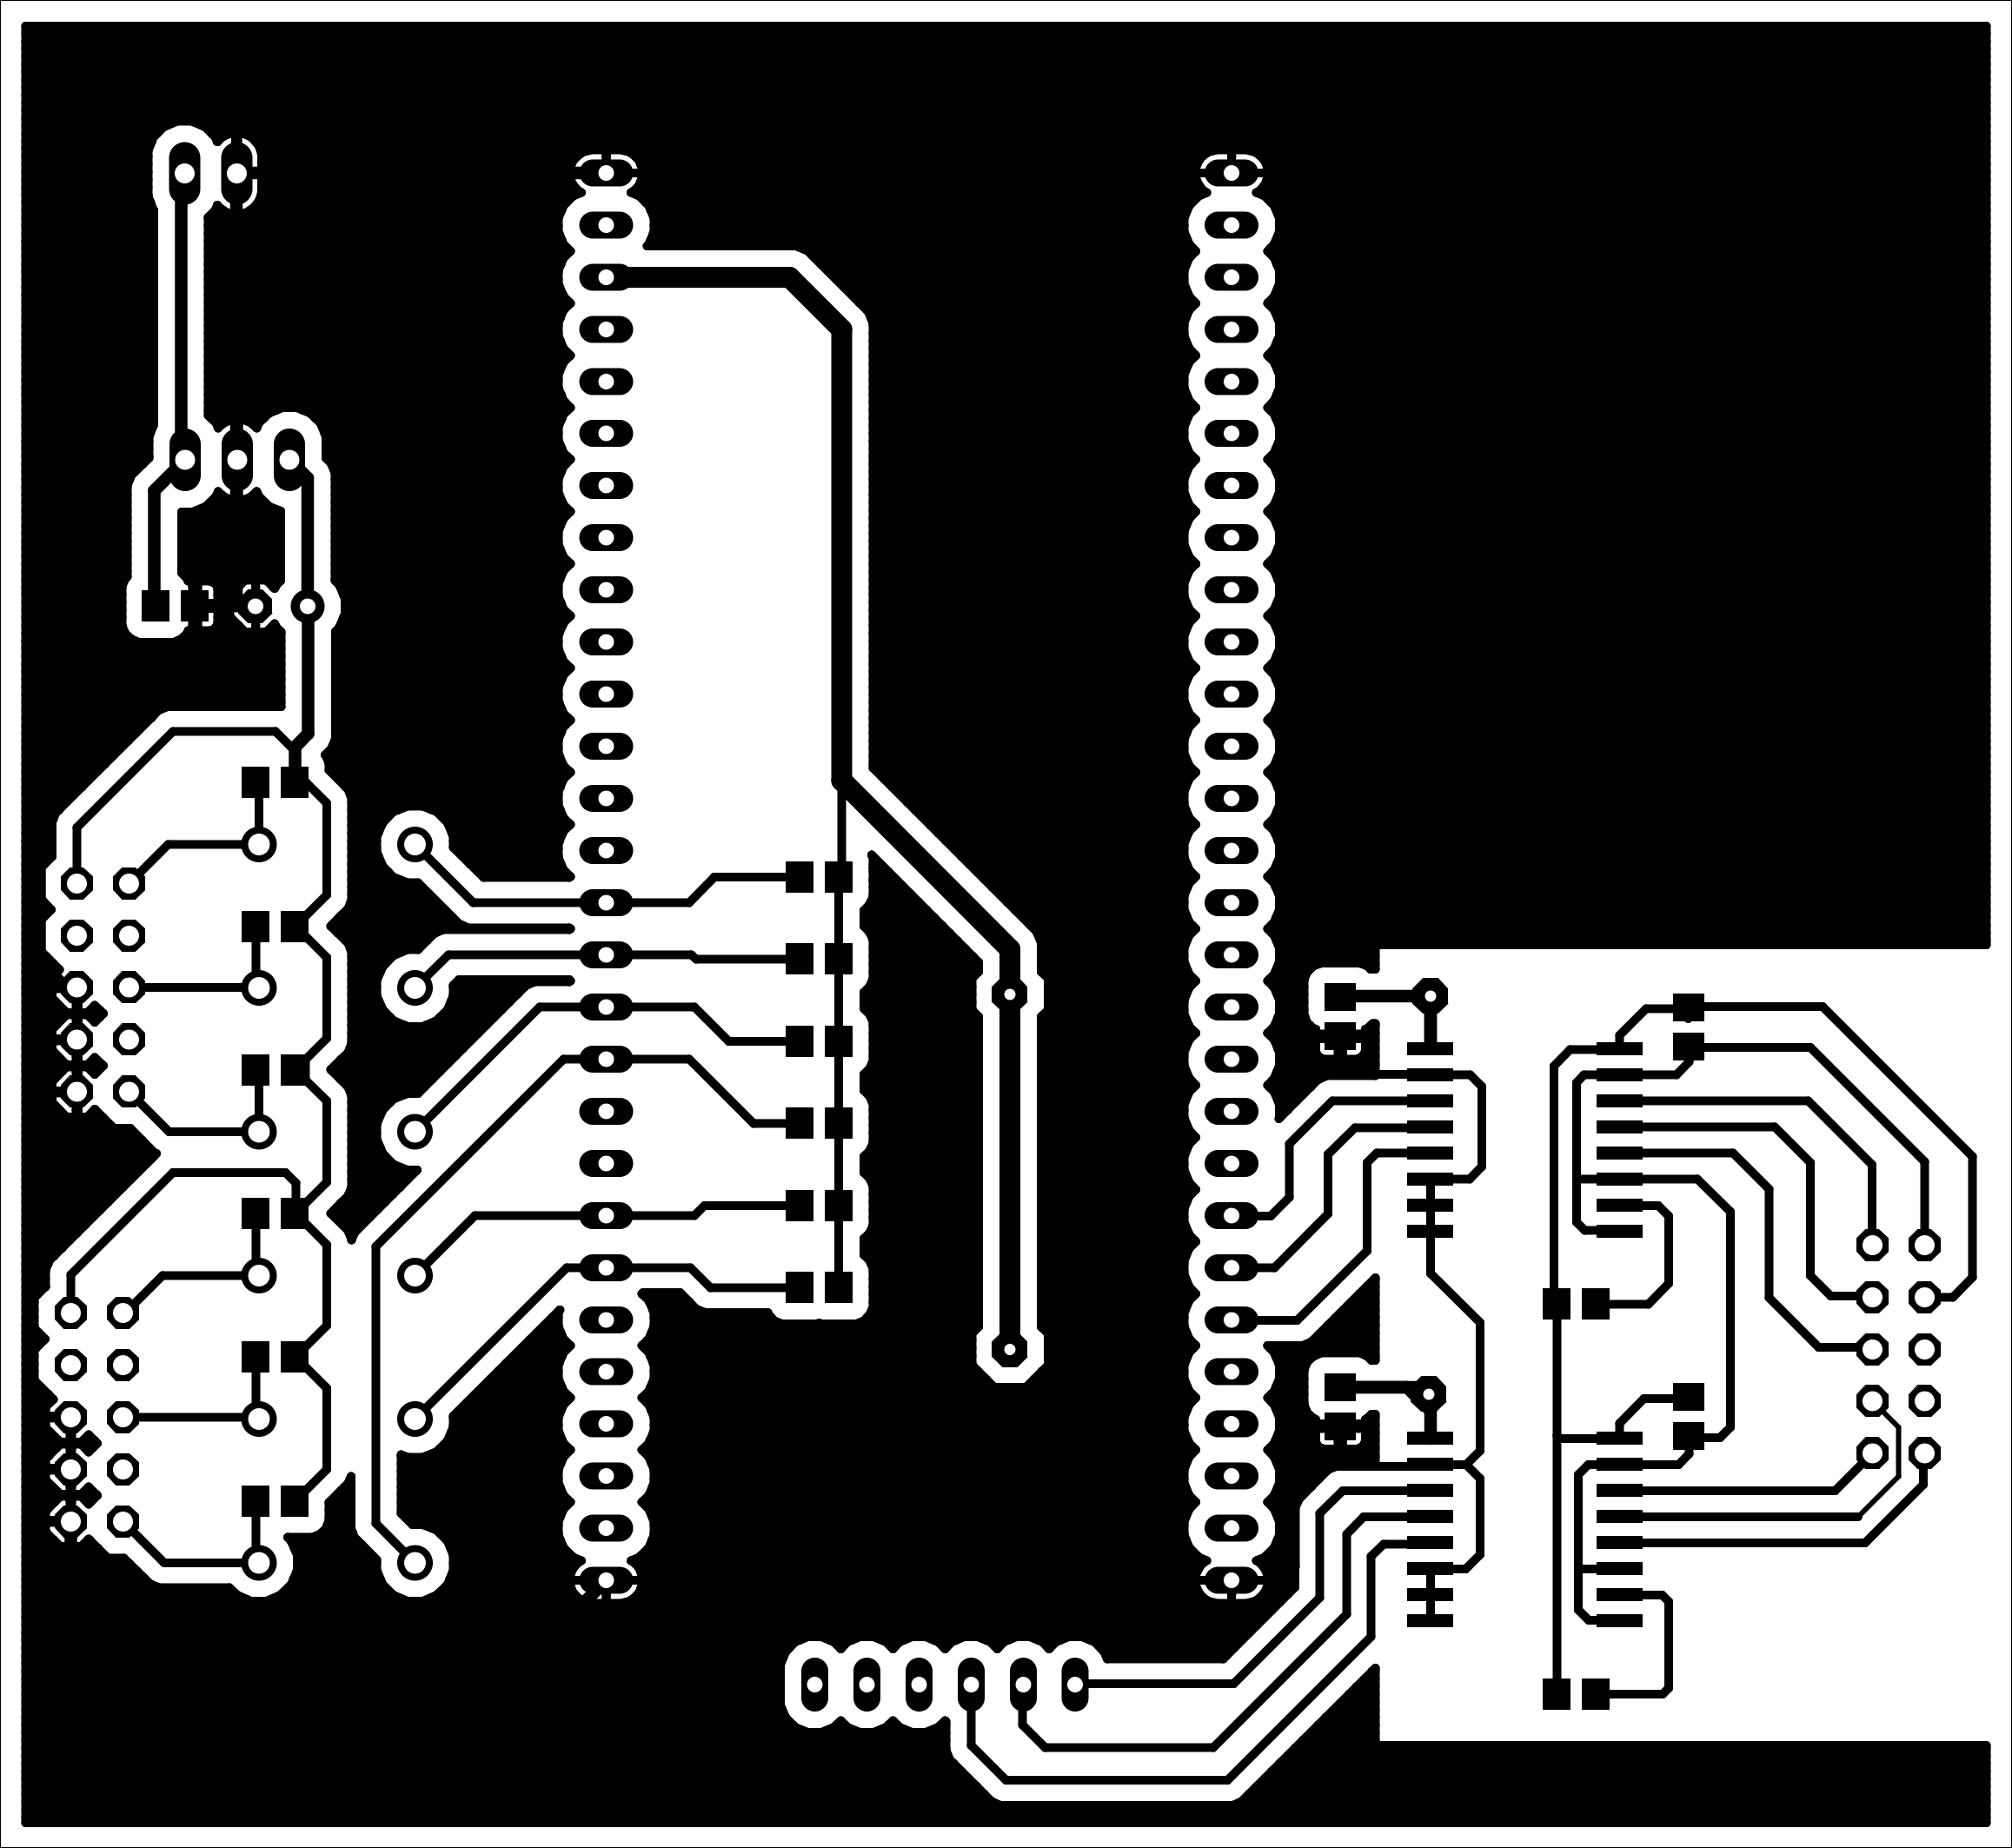
\includegraphics[width=0.8\linewidth]{img/control-board-route}}
            \caption{Чертеж печатной платы блока управления АИН}
            \label{fig:control-board-route}
        \end{figure}

        \begin{figure}[h!]
            \center{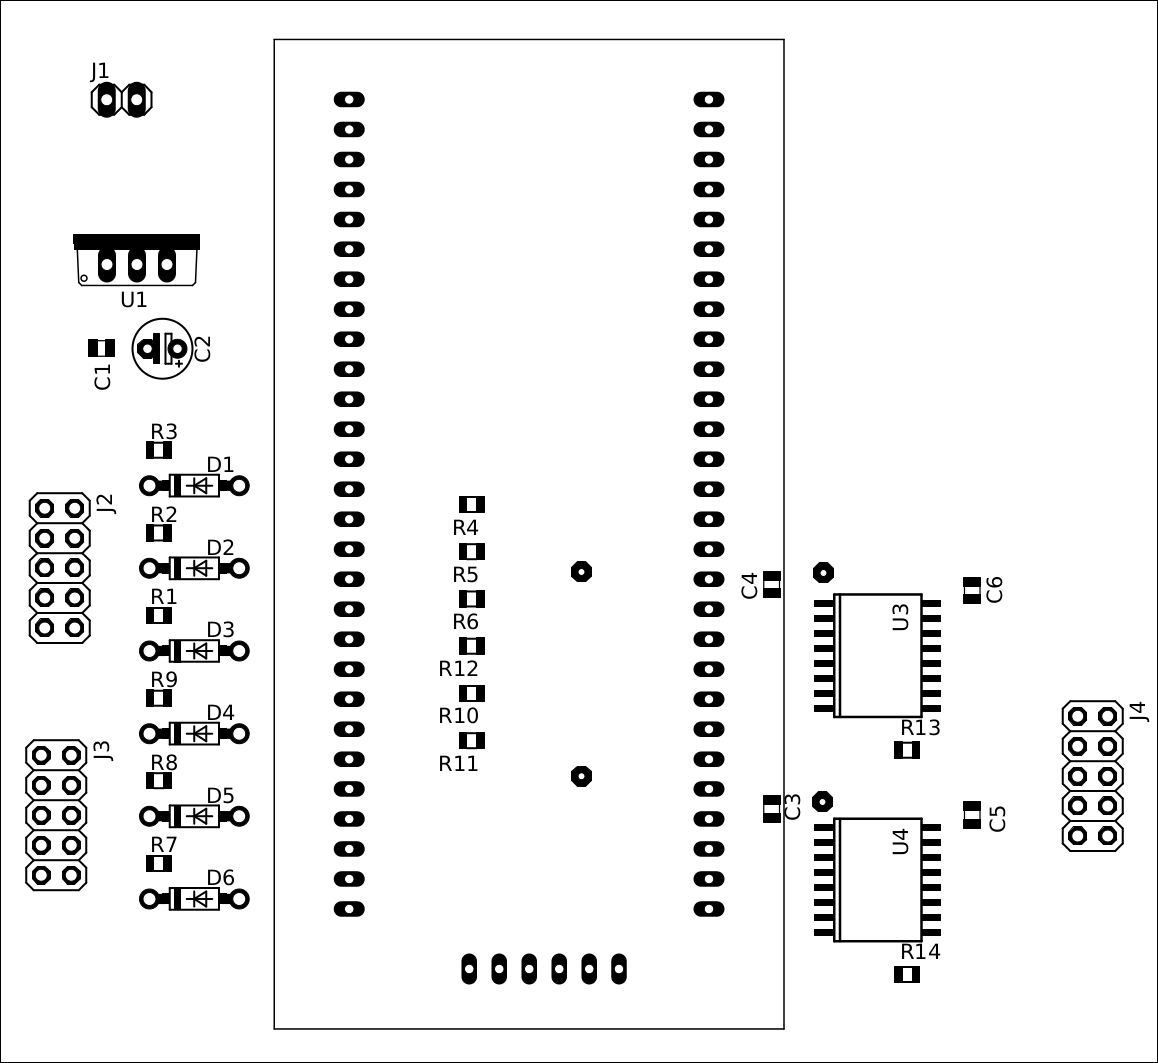
\includegraphics[width=0.8\linewidth]{img/control-board-place}}
            \caption{Схема расположения элементов блока управления АИН}
            \label{fig:control-board-place}
        \end{figure}
        
    \subsubsection{Описание модуля STM32VLDiscovery}
        STM32VLDiscovery -- встраиваемый модуль с интегрированным\\
        JTAG-отладчиком на базе микроконтроллера STM32F100RBT6B семейства STM32
        Value Line. Работа с платой поддерживается в интегрированной среде
        разработки компаний IAR, Keil, Atollic, а также свободным набором
        компиляторов GNU Compiler Collection.

        Установленный микроконтроллер в 64-выводном корпусе LQFP работает на
        частоте 24 МГц. Плата имеет разъем расширения, который позволяет
        подключать ее к другим отладочным платформам для более глубокого
        анализа работы периферии микроконтроллера или к макетным платам для
        прототипирования.

        Установленный на плате отладчик/программатор ST-Link, может
        использоваться как для внутрисхемного программирования встроенного
        микроконтроллера так и в качестве отдельного устройства.

        Отличительные особенности:
        \begin{itemize}
            \item на плате имеется внутрисхемный отладчик/программатор ST-Link;
            \item USB интерфейс ко встроенному отладчику;
            \item переключатель для использования платы в качестве отдельного
                устройства ST-Link;
            \item питание возможно от USB интерфейса или от внешнего источника; 
            \item два светодиода индикации состояния;
            \item два пользовательских светодиода, пользовательская кнопка,
                кнопка \\ <<Сброс>>;
            \item коннектор расширения – доступны все линии ввода/вывода
                микроконтроллера, может использоваться для подключения к
                макетной плате или другой отладочной системе.
        \end{itemize}

        Внешний вид, расположение элементов и размеры модуля приведены на
        рисунке \ref{fig:stm32vldiscovery}.

        \begin{sidewaysfigure}
            \center{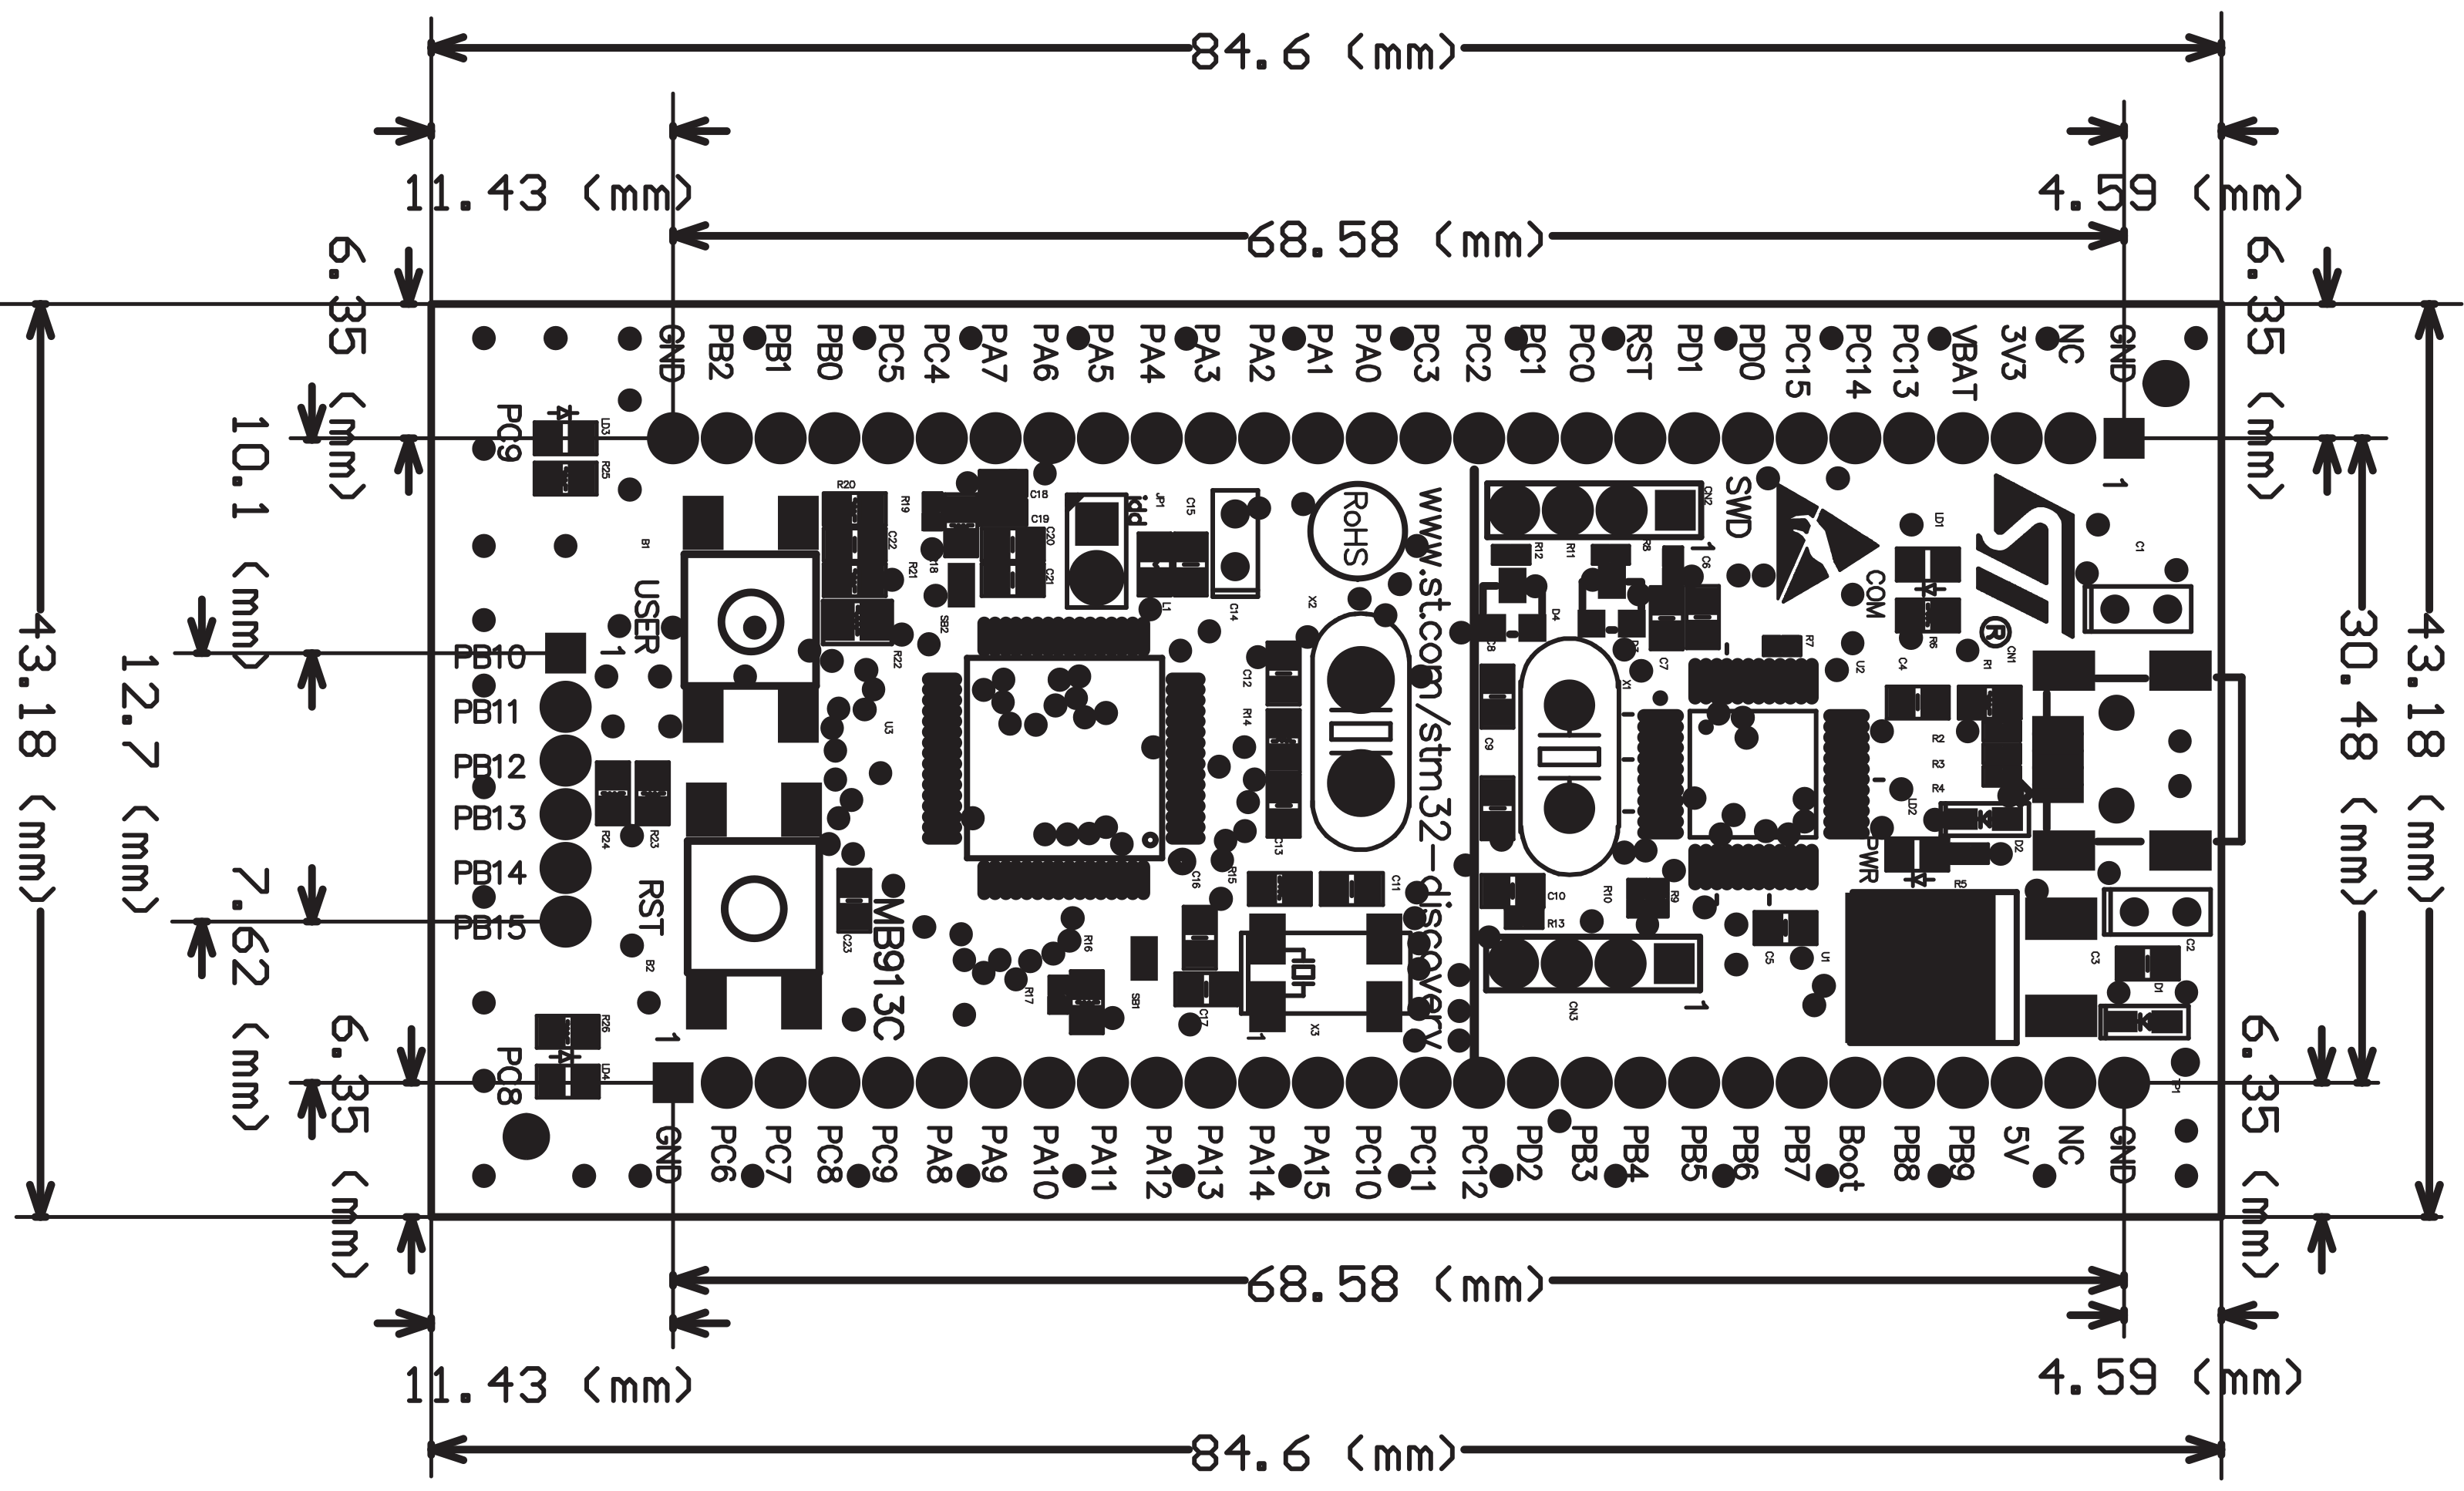
\includegraphics[width=0.8\linewidth]{img/stm32vldiscovery}}
            \caption{Размеры и расположение элементов модуля STM32VLDiscovery}
            \label{fig:stm32vldiscovery}
        \end{sidewaysfigure}       

    \subsubsection{Описание микроконтроллера STM32F100RBT6B}
        Особенности микроконтроллера STM32F100R:
        \begin{itemize}
            \item Вычислительное ядро Cortex-M3;
            \item Максимальная тактовая частота: 24 МГц;
            \item Напряжение питания 2,0 — 3,6 В;
            \item 128 кбайт NOR flash памяти с количеством циклов перезаписи 10000;
            \item 8 кбайт статической оперативной памяти;
            \item 7-канальный контроллер прямого доступа в память;
            \item 51 линия портов ввода-вывода общего назначения;
            \item 12-битный 16-канальный АЦП с временем преобразования 1,2 мкс;
            \item 12-битный ЦАП;
            \item 16-битный таймер с расширенными функциями;
            \item шесть 16-битных таймеров общего назначения;
            \item Восемь коммуникационных интерфейсов (I2C, USART, SPI).
        \end{itemize}

        \begin{sidewaysfigure}
            \center{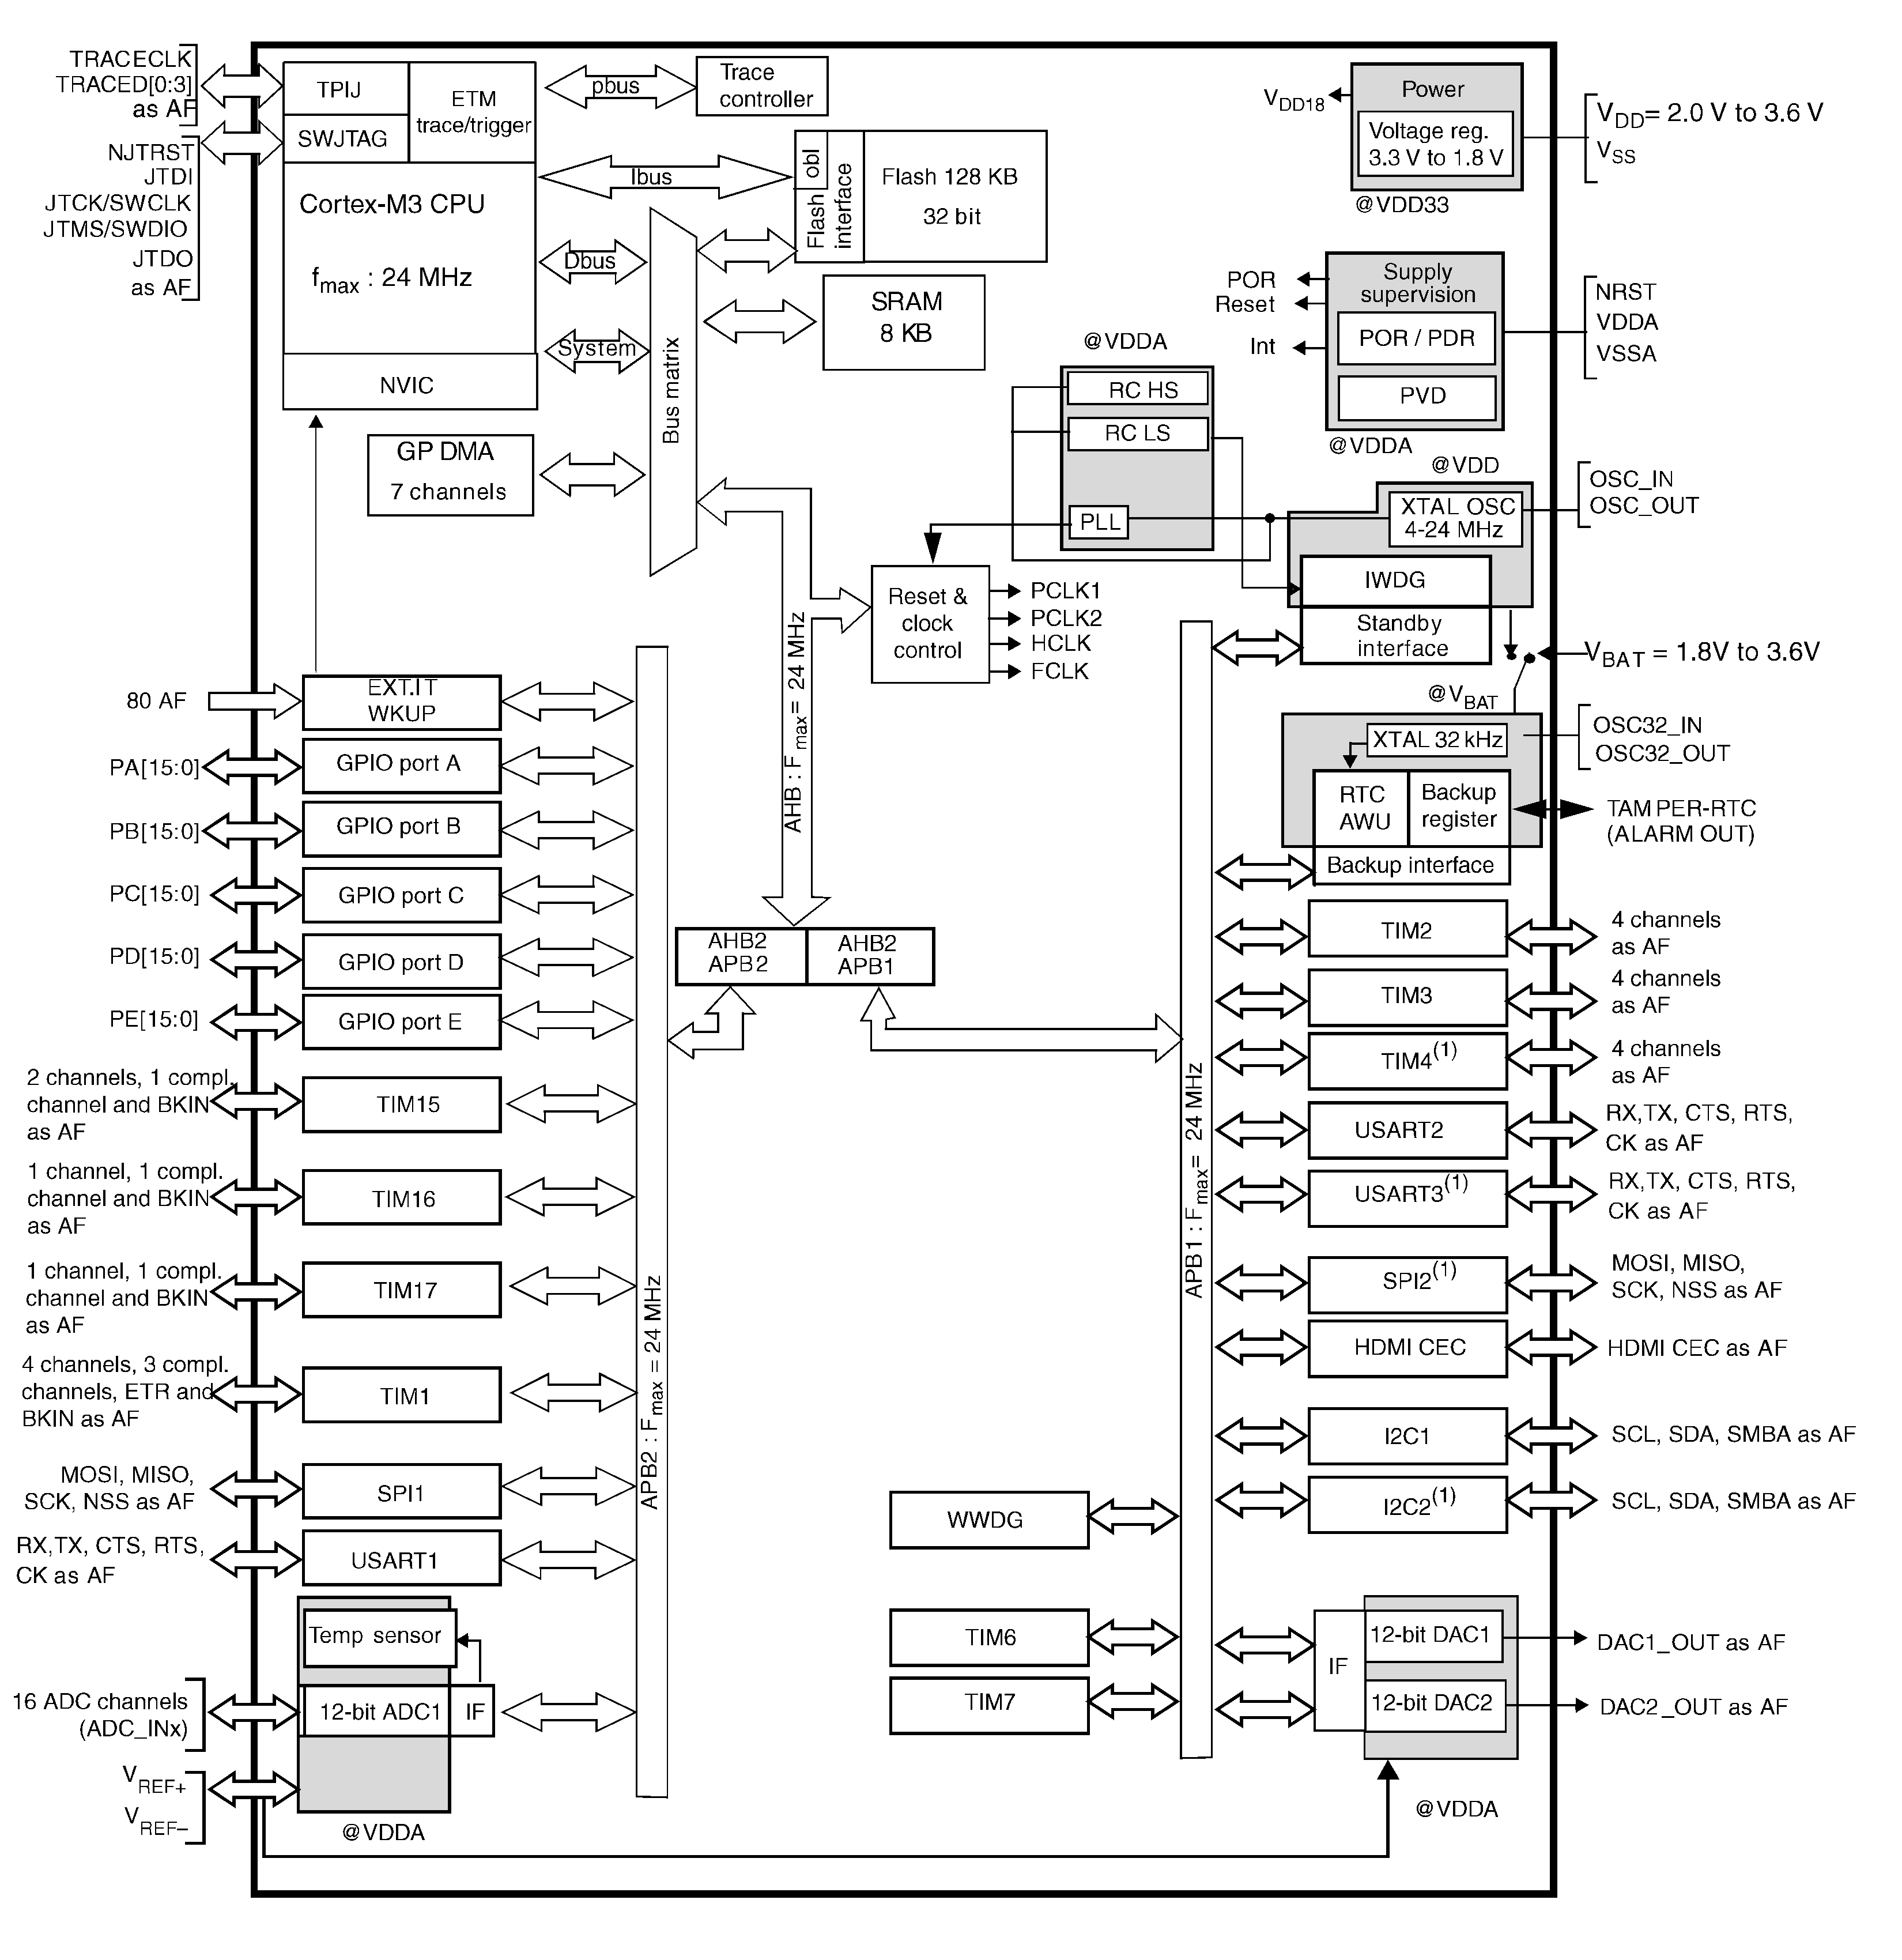
\includegraphics[width=0.65\linewidth]{img/stm32f100rbt6b}}
            \caption{Структурная схема микроконтроллера STM32F100RBT6B}
            \label{fig:stm32f100rbt6b}
        \end{sidewaysfigure}       
        
        Контроллер основан на высокопроизводительном 32 битном вычислительном
        ядре Cortex-M3 фирмы ARM.

        Cortex-M3 является стандартизованным микроконтроллерным ядром, которое
        помимо ЦПУ, содержит все остальные составляющие основу микроконтроллера
        элементы (в том числе приоритетный контроллер вложенных прерываний, 24
        битный системный таймер, интегрированный в ядро отладочный интерфейс). 

        4 гигабайтное адресное пространство Cortex-M3 разделено на четко
        распределенные области кода программы, статического ОЗУ, устройств
        ввода-вывода и системных ресурсов. Cortex-M3 выполнено по Гарвардской
        архитектуре и  имеет несколько шин, позволяющие параллельно выполнять
        такие операции как загрузка опкода, его выполнение (у МК имеется
        трехступенчатый конвеер), перемещение данных между регистрами и ОЗУ.

        Центральный процессорный элемент ядра Cortex-M3 имеет 13 регистров
        общего назначения, аппаратный 32 битный одноцикловый перемножитель,
        аппаратный делитель, а так же поддерживает два режима работы: потоковый
        режим (Thread) и режим обработчика (Handler), для каждого из которых
        можно сконфигурировать свои собственные стеки. Благодаря этому,
        появляется возможность разработки более интеллектуального программного
        обеспечения и поддержки операционных систем реального времени (ОСРВ) не
        только с кооперативной, но и с вытесняющей многозадачностью.

        Контроллер векторизированных вложенных прерываний (КВВП) может
        обрабатывать до 255 векторов, включая 15 исключений генерируемых
        процессорным ядром. КВВП также позволяет установить каждому вектору
        один из 16 уровней приоритета.

        Вход в процедуру обработки прерывания длится всего 12 машинных
        циклов, а на обработку каждого следующего вложенного прерывания
        процессор использует всего 6 циклов. Это достигнуто  за счет
        автоматического сохранения контекста прерванной программы и
        переключения стеков, выполняемых специальным микрокодом внутри ЦПУ.

        В ядро Cortex-M3 также входит 24-битный автоматически перезагружаемый
        таймер, предназначенный для генерации периодических прерываний и
        используемый ядром ОСРВ.

        Микроконтроллер имеет 16-битный таймер с возможностью управления
        трехфазным мостом силовых транзисторов. Таймер обеспечивает
        программируемое мертвое время, вход аварийной блокировки,
        настраиваемую полярность ШИМ сигнала.

        Два таймера общего назначения позволяют осуществлять обработку данных
        инкрементных энкодеров. Вычисление положения вала электродвигателя
        работает полнотью автоматически, независимо от ядра микроконтроллера.

        Семиканальный контроллер прямого доступа в память играет важную роль при
        программировании интерфейсов передачи данных, помогая существенно разгрузить
        вычислительное ядро.

        Хотя напряжение питания микроконтроллера 3,3В, практически все его
        порты ввода-вывода толерантны к напряжениям до 5В.

    \subsubsection{Описание цифровых изоляторов ADUM1300}
        ADuM1300 – трех канальные цифровые изоляторы компании Analog Devices.
        Отличительные особенности:
        \begin{itemize}
            \item низкое потребление (1.0 мА на канал на скорости до 10
                Мбит/с);
            \item двунаправленная передача данных;
            \item совместим с 3.3 В и 5.0 В питанием/уровнями логических
                сигналов;
            \item высокая скорость передачи данных: от 0 до 10 Мбит/с;
            \item максимальное искажение длительности импульса 2 нс;
            \item максимальное временное рассогласование каналов 2 нс;
            \item способность выдерживать воздействие изменяющегося входного
                синфазного сигнала, имеющего скорость нарастания более 25
                кВ/мкс;
            \item Функция активизации выходов;
            \item широкий 16 выводной SOIC корпус;
        \end{itemize}

        \begin{figure}[h!]
            \center{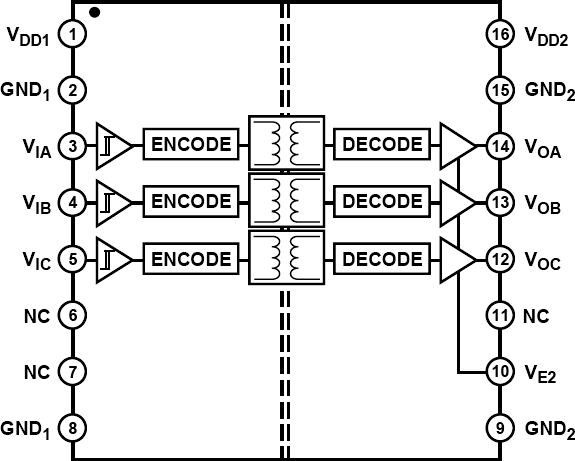
\includegraphics[width=0.8\linewidth]{img/adum1300}}
            \caption{Структурная схема цифрового изолятора ADUM1300}
            \label{fig:adum1300}
        \end{figure}

        Изоляторы семейства ADUM130X имеют три независимых канала и выпускаются
        в трех модификациях с различной пропускной способностью. Прибора
        ADuM1300 работает от однополярного источника питания, подключенного к
        любой стороне прибора, от 2,7 до 5,5 В, что позволяет обеспечить
        совместимость с низковольтными системами и произвести преобразование
        уровней сигналов через изоляционный канал. Кроме того, приборы ADUM130X
        обеспечивают низкие искажение ширины импульсов и временное
        рассогласование каналов.  Изоляторы ADUM130X имеют запатентованную
        функцию регенерации, которая гарантирует передачу статических
        параметром логических сигналов.

    \subsection{Разработка и реализация программной части системы управления АИН}
        Управляющее программное обеспечение электропривода
        лабораторно-исследовательского стенда полностью реализовано на языке C
        согласно стандарту С89. Компиляция осуществлялаь пакетом программ ARM
        GCC из набора GNU Compiler Collection. Автоматизация сборки реализована
        средствами GNU Make.

        Контроль версий производиться с помощью систмы Git. Репозиторий
        исходного кода расположен по адресу
        https://github.com/reviakinea/acid.git.

    \subsubsection{Программный синтез трехфазной системы синусоидальных напряжений}
        Под термином <<синтезатор частоты>> понимают электронное устройство,
        способное из опорной частоты получать на выходе требуемую частоту или
        набор частот,  согласно управляющим сигналам.

        DDS  уникальны своей цифровой определенностью:  генерируемый ими сигнал
        синтезируется со свойственной цифровым системам точностью.  Частота,
        амплитуда и фаза сигнала в любой момент времени точно известны и
        подконтрольны. DDS  практически не подвержены температурному дрейфу и
        старению.

        Основные преимущества DDS:  
        \begin{itemize}
            \item цифровое управление частотой и фазой выходного сигнала;
            \item очень высокое разрешение по частоте и фазе;
            \item экстремально быстрый переход на другую частоту (или фазу),
                перестройка по частоте без разрыва фазы,  без выбросов и других
                аномалий,  связанных с временем установления;
            \item архитектура,  основанная на DDS,  ввиду очень малого шага
                перестройки по частоте, исключает необходимость применения
                точной подстройки опорной частоты,  а также обеспечивает
                возможность параметрической температурной компенсации;
        \end{itemize}

        Частотное разрешение DDS  составляет сотые,  и даже тысячные доли герца
        при выходной частоте порядка десятков мегагерц.  Такое разрешение
        недостижимо для других методов синтеза. Другой характерной особенностью
        DDS  является очень высокая скорость перехода на другую частоту.  Более
        того,  все перестройки по частоте происходят у DDS  без разрыва фазы
        выходного сигнала.  Поскольку выходной сигнал синтезируется в цифровом
        виде,  очень просто осуществить модуляцию различных видов.

        Упрощенная блок-схема генератора прямого цифрового синтеза сигналов
        приведена на рисунке \ref{fig:dds-structure}. 

        \begin{figure}[h!]
            \center{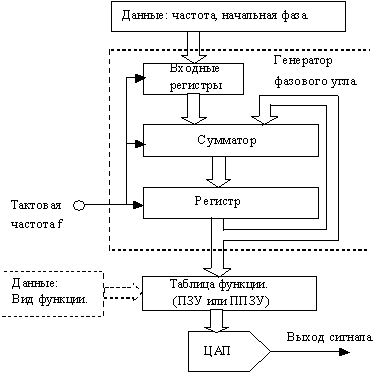
\includegraphics[width=0.55\linewidth]{img/dds-structure}}
            \caption{Структурная схема прямого цифрового синтеза частоты}
            \label{fig:dds-structure}
        \end{figure}

        Схема содержит три основных блока: генератор фазового угла, память и
        ЦАП. Генератор фазового угла в типичном случае представляет собой
        накапливающий сумматор с регистром. Работает он просто как регистр
        фазы, содержимое которого получает приращение на некоторый фазовый угол
        через заданные интервалы времени. Приращение фазы и её начальное
        значение загружаются в виде цифровых кодов во входные регистры. Память
        играет роль таблицы функций. Код текущей фазы поступает на ее адресные
        входы, а с выхода данных на вход цифроаналогового преобразователя
        поступает код, соответствующий текущему значению заданной функции.  ЦАП
        в свою очередь формирует аналоговый сигнал. В системе электропривода в
        роли ЦАП выступает генератор ШИМ сигнала и силовой блок АИН.

        Регистр содержит текущую фазу выходного сигнала в виде целого числа,
        которое при каждом тактовом импульсе получает приращение $\Delta n$,
        также целое число. Таким образом, текущий аргумент функции
        представляется целым числом Tn по модулю $2^N$, где $N$ -разрядность
        сумматора. Т.е.  последовательность значений аргумента является
        квазипериодической функцией. Дискретность по времени определяется
        тактовой частотой fc.  Увеличение разрядности регистра повышает
        разрешающую способность приращения аргумента $\Delta n$. Значения
        функции округляются в соответствии с разрядностью ЦАП.

        Так как производится синтез гармонического колебания, фазовый угол
        $\varphi$ равен: $\varphi = 2\pi \cdot T_n$. Тогда частота выходного
        сигнала $F$ равна произведению частоты тактов $F_{DDS}$ на относительное
        приращение целочисленного аргумента:
        \begin{gather*}
            F = \frac{\Delta n \cdot F_{DDS}}{2^N}.
        \end{gather*}

        Листинг функии синтеза трехфазной системы напряжений:
        \begin{verbatim}
        void sine_generation_task(void)
        {
            uint8_t  index;
            uint16_t pwm;

            /* phase increment */
            m_phase += m_delta;
         
            /* phase U duty cycle */
            index = (m_phase + PHASE_SHIFT_U) >> 8;
            pwm = (sine_table[index] * m_amplitude) >> 7;

            pwm_load_u(PWM_ZERO + pwm);

            /* phase V duty cycle */
            index = (m_phase + PHASE_SHIFT_V) >> 8;
            pwm = (sine_table[index] * m_amplitude) >> 7;

            pwm_load_v(PWM_ZERO + pwm);

            /* phase W duty cycle */
            index = (m_phase + PHASE_SHIFT_W) >> 8;
            pwm = (sine_table[index] * m_amplitude) >> 7;

            pwm_load_w(PWM_ZERO + pwm);
        }
        \end{verbatim}

        В приведенном выше листинге роль накапливающего сумматора фазы играет
        16-битная переменная \verb"m_phase". На каждой итерации системы эта
        переменная получает приращение фазы $\Delta n$, которое храниться в
        \verb"m_delta". Аккумулятор фазы обеспечивает арифметику по модулю
        $2^{16}$, что соответствует переодичности функции синуса.

        Далее, из таблицы значений функции синуса (индекс в таблице
        соответствует восьми старшим переменной \verb"m_phase") выбирается
        значение и перемножается на амплитуду. Эта последовательность
        повторяется для остальных двух фаз, за исключением сдвига фазы сигнала.

        На вход блока синтеза трехфазной системы синусоидальных напряжений
        поступают два сигнала: амплитуда сигнала $A$ (в переменной
        \verb"m_amplitude") и приращение фазы $\Delta n$ (в переменной
        \verb"m_delta"). Частота выходного сигна определяется по формуле:
        \begin{gather*}
            F = \frac{\Delta n \cdot F_{DDS}}{2^{16}},
        \end{gather*}

        где $F_c$ -- частота следования итераций алгоритма (в данном случае $F_{DDS} = 12$ КГц).

        Амплитуда выходного сигнала:
        \begin{gather*}
            A_\text{вых} = \frac{U_\text{п} \cdot A}{2000},
        \end{gather*}

        где $U_\text{п}$ -- выпрямленное напряжение питания инвертора. 

%        ШИМ сигнал управления трехфазным мостом АИН формируется блоком
%        сравнения таймера 1 микроконтроллера.
    \subsubsection{Релизация скалярного закона управления}
        Закон управления $V/f = const$ реализован в функции, листинг которой приведен ниже:
        \begin{verbatim}
            unsigned int vf_control(int frequency)
            {
                unsigned int amplitude;

                frequency = abs(frequency);

                /* Vf law */
                amplitude = frequency * VF_SLOPE / 256;

                /* Amplitude saturation */
                if (amplitude > VF_MAX_AMPLITUDE)
                {
                    amplitude = VF_MAX_AMPLITUDE;
                } 
                else if (amplitude < VF_MIN_AMPLITUDE)
                {
                    amplitude = VF_MIN_AMPLITUDE;
                }

                return amplitude;
            }
        \end{verbatim}
        
        Входным параметром данной функции является частота синусоидального
        сигнала. В соответствии со входным параметром и наклоном
        характеристики, заданным константой \verb"VF_SLOPE", функция возвращает
        необходимое напряжение питания статора электродвигателя. Выходное
        значение, также, ограничивается в пределах значения констант
        \verb"VF_MIN_AMPLITUDE" и \verb"VF_MAX_AMPLITUDE".
        
        Значение константы \verb"VF_SLOPE" определяется следующим отношением:
        \begin{gather*}
            V/f = \frac{U_\text{н}}{f_\text{н}} \cdot \frac{K_{DDS}}{2000} \cdot 256,
        \end{gather*}

        где $U_\text{н}$ -- номинальное напряжение питания электродвигателя;\par
        $f_\text{н}$ -- номинальная частота питающего напряжения электродвигателя;\par
        $K_{DDS}$ -- коэффициент передачи модуля синтеза частоты.

        Коэффициент передачи синтезатора определяется так:
        \begin{gather*}
            K_{DDS} = \frac{F_{DDS}}{2^{16}},
        \end{gather*}

        где $F_{DDS}$ -- частота приращения фазы синтезатора (в данном случае
        $F_{DDS} = 12$ КГц).

        Для данного двигателя наклон прямой зависимости напряжения питания от
        частоты выражается следующей формулой:
        \begin{gather*}
            V/f = \frac{220}{50} \cdot \frac{12000}{2^{16}} \cdot 256 = 206
        \end{gather*}

    \subsection{Реализация дискретного ПИД-регулятора}
        Для стабилизации скорости частоты вращения вала электродвигателя был
        применен дискретный ПИД-регулятор. Регулятор реализован программно
        внутри управляющего ПО системы электропривода.

        \begin{figure}[h!]
            \center{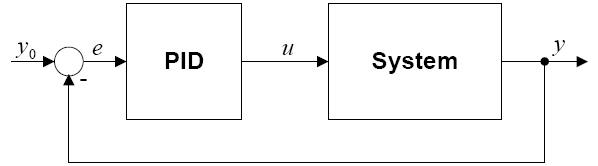
\includegraphics[width=0.8\linewidth]{img/system-with-pid}}
            \caption{Структурная схема системы с ПИД-регулятором}
            \label{fig:system-with-pid}
        \end{figure}

        На рисунке \ref{fig:system-with-pid} показана схема системы с
        ПИД-регулятором. На вход ПИД-регулятора поступает значение частоты
        вращения ротора электродвигателя, снятое с датчика скорости. Регулято
        сравнивает измеренное значение частоты вращения  с заданным опорным
        значением. Затем разница, или ошибка, E, обрабатывается для расчета
        сигнала задания. Этот сигнал задания будет пытаться приблизить значение
        измеряемого параметра (частоты вращения вала) к заданному значению.

        Альтернативой системе управления с замкнутым контуром, является система
        управления с открытым контуром. Применение открытого контура управления
        (без обратной связи) в данном случае не является удовлетворительным.

        В отличие от простых алгоритмов управления, ПИД-регулятор способен
        управлять процессом, основываясь на его истории и скорости изменения.
        Это дает более точный и стабильный метод управления.

        Структурная схема ПИД-регулятора показана на рисунке \ref{fig:pid}, где
        $T_p$, $T_i$, и $T_d$ обозначают постоянные времени пропорциональной,
        интегральной, и дифференциальной составляющих соответственно.

        Передаточная функция системы, изображенной на рисунке \ref{fig:pid}
        имеет вид:
        \begin{gather*}
            \frac{u}{e}(s) = H(s) = K_p \left(1 + \frac{1}{T_i s} + T_d s\right).
        \end{gather*}

        Отсюда имеем:
        \begin{gather*}
            u(t) = K_p \left( e(t)+\frac{1}{T_i} 
                \int \limits_0^t e(\sigma)d \sigma + T_d \frac{de(t)}{dt} \right).
        \end{gather*}

        Пропорциональная составляющая (П) дает управляющий сигнал
        пропорционально вычисленной ошибке. Использование только одного
        пропорционального управления дает стационарную ошибку всегда, кроме
        случаев, когда управляющий сигнал равен нулю, а значение системного
        процесса равно требуемой величине.Использование слишком большого
        П-члена даст неустойчивую систему. 

        Интегральная составляющая (И) представляет собой предыдущих ошибок.
        Суммирование ошибки будет продолжаться до тех пор, пока значение
        системного процесса не станет равно нужному значению. Обычно
        интегральную составляющую используют вместе с пропорциональной, в так
        называемых ПИ-регуляторах. Использование только интегральной
        составляющей дает медленный отклик и часто колебательную систему.
        Отклик ПИ-регулятора не имеет стационарной ошибки, а отклик
        И-регулятора очень медленной.

        Дифференциальная составляющая (Д) представляет собой скорость изменения
        ошибки. Добавление этой составляющей улучшает отклик системы на
        внезапное изменение ее состояния. Дифференциальная составляющая Д
        обычно используется с П или ПИ алгоритмами, как ПД или ПИД контроллеры.
        Большая дифференциальная составляющая Д обычно дает неустойчивую
        систему. Отклик ПД-контроллера дает быстрый рост значения процесса, чем
        П контроллер. Обратите внимание, что дифференциальная составляющая Д
        ведет себя по существу как фильтр верхних частот для сигнала ошибки и,
        таким образом легко делает систему нестабильной и более чувствительной
        к шуму.

        Аппроксимируем интегральную и дифференциальную составляющие, чтобы
        получить дискретный вид:
        \begin{gather*}
            \int \limits_0^t e(\sigma)d\sigma \approx T \sum \limits_{k=0}^n e(k),\\
            \frac{de(t)}{dt} \approx \frac{e(n) - e(n - 1)}{T},\\
            t = nT,
        \end{gather*}

        где $n$ -- дискретный шаг времени t.

        Это дает нам такой регулятор:
        \begin{gather*}
            u(n) = K_p e(n) + K_i \sum \limits_{k=0}^n e(k) + K_d (e(n)-e(n-1));
        \end{gather*}

        Где
        \begin{gather*}
            K_i = \frac{K_p T}{T_i};\\
            K_d = \frac{K_p T_d}{T}.
        \end{gather*}

        Реализация ПИД-контоллера на языке С представлена ниже:
        \begin{verbatim}
            #define SCAL_FACTOR 1024
            #define P_TERM_MAX  (INT32_MAX / 4)
            #define I_TERM_MAX  (INT32_MAX / 4)

            typedef struct {

                /* PID koeff. */
                uint16_t    p_factor;
                uint16_t    i_factor;
                uint16_t    d_factor;

                /* Int. term summator */
                int32_t     sum_error;

                /* Last measured value. Use for diff. term */
                int16_t     last_meas;

                /* Max values */
                int32_t     max_sum;
                int32_t     max_error;
            } pidc_t;
            void pid_init( pidc_t *pid, uint16_t p_factor,
                uint16_t i_factor, uint16_t d_factor )
            {
                /* Reset PID */
                pid->last_meas = 0;
                pid->sum_error = 0;

                /* Tuning */
                pid->p_factor = p_factor;
                pid->i_factor = i_factor;
                pid->d_factor = d_factor;

                /* Calculate max values */
                pid->max_error = P_TERM_MAX / (pid->p_factor + 1);
                pid->max_sum   = I_TERM_MAX / (pid->i_factor + 1);
            }
            int16_t pid_controller( pidc_t *pid, 
                int16_t ref, int16_t meas )
            {
                int32_t p_term, i_term, d_term;
                int32_t error, temp;

                error = ref - meas;

                if ( error > pid->max_error ) {
                    p_term = P_TERM_MAX;
                } else if ( error < -pid->max_error ) {
                    p_term = -P_TERM_MAX;
                } else {
                    p_term = pid->p_factor * error;
                }

                temp = pid->sum_error + error;
                if ( temp > pid->max_sum ) {
                    i_term = I_TERM_MAX;
                } else if ( temp < -I_TERM_MAX ) {
                    i_term = -I_TERM_MAX;
                } else {
                    pid->sum_error = temp;
                    i_term = pid->i_factor * pid->sum_error;
                }

                d_term = pid->d_factor * pid->last_meas - meas;
                pid->last_meas = meas;

                return (int16_t) ((p_term + i_term + d_term) 
                    / SCAL_FACTOR);
            }
        \end{verbatim}

        Все данные ПИД-регулятора хранятся в структуре \verb"pidс_t". Функция\\
        \verb"pid_init()" получает на вход коэффициенты регулятора и
        инициализирует структуру ПИД. Функция \verb"pid_controller()" вычисляет
        сигнал управляющего воздействия по переданным ей значениям сигнала
        задания и измереного значения частоты вращения.

    \subsubsection{Реализация протокола передачи данных Modbus RTU}
        Для взаимодействия с управляющим персональным копьютером в программное
        обеспечение системы управления был добавлен алгориитм, реализующий
        стандартизированный бинарный протокол передачи данных Modbus RTU. Выбор
        протокола передачи данных основан на простоте реализации и многообразии
        уже написанного ПО для отладки и обмена данными по этому протоколу.

        Modbus — открытый коммуникационный протокол, основанный на архитектуре
        <<клиент-сервер>>. Широко применяется в промышленности для организации
        связи между электронными устройствами. Может использоваться для
        передачи данных через последовательные линии связи RS-485, RS-422,
        RS-232, а также сети TCP/IP (Modbus TCP).

        Контроллеры на шине Modbus взаимодействуют, используя клиент-серверную
        модель, основанную на транзакциях, состоящих из запроса и ответа.

        Обычно в сети есть только один клиент, так называемое, <<главное>> 
        (master) устройство, и несколько серверов — <<подчиненных>> (slaves)
        устройств. Главное устройство инициирует транзакции (передаёт запросы).
        Главный может адресоваться индивидуально к подчиненному или
        инициировать передачу широковещательного сообщения для всех подчиненных
        устройств. Подчиненное устройство отвечает на запрос, адресованный
        именно ему. При получении широковещательного запроса ответ не
        формируется.

        Спецификация Modbus описывает структуру запросов и ответов. Их основа —
        элементарный пакет протокола, так называемый PDU (Protocol Data Unit).
        Структура PDU не зависит от типа линии связи и включает в себя код
        функции и поле данных. Код функции кодируется однобайтовым полем и
        может принимать значения в диапазоне 1..127. Диапазон значений 128..255
        зарезервирован для кодов ошибок. Поле данных может быть переменной
        длины. Размер пакета PDU ограничен 253 байтами.

        Для передачи пакета по физическим линиям связи PDU помещается в другой
        пакет, содержащий дополнительные поля. Этот пакет носит название ADU
        (Application Data Unit).Общая структура ADU следующая:
        
        \begin{itemize}
            \item адрес ведомого устройства — адрес подчинённого устройства, к
                которому адресован запрос. Ведомые устройства отвечают только
                на запросы, поступившие в их адрес. Ответ также начинается с
                адреса отвечающего ведомого устройства, который может
                изменяться от 1 до 247. Адрес 0 используется для
                широковещательной передачи, его распознаёт каждое устройство,
                адреса в диапазоне 248..255 — зарезервированы; 
            \item код функции — это следующее однобайтное поле кадра. Оно
                говорит ведомому устройству, какие данные или выполнение какого
                действия требует от него ведущее устройство; 
            \item данные — поле содержит информацию, необходимую ведомому
                устройству для выполнения заданной мастером функции или
                содержит данные, передаваемые ведомым устройством в ответ на
                запрос ведущего.  Длина и формат поля зависит от номера
                функции;
            \item блок обнаружения ошибок — контрольная сумма для проверки
                отсутствия ошибок в кадре.
        \end{itemize}

        Максимальный размер ADU для последовательных сетей RS232/RS485 — 256
        байт, для сетей TCP — 260 байт. 

        Ошибки передачи данных обнаруживаются при помощи фреймов символов,
        контроля чётности и циклической контрольной суммы CRC-16-IBM
        (используется число-полином = 0xA001). 

        Наличее в микроконтроллере контроллера прямого доступа в память
        позволило реализовать очень быстрый и нетребовательный к ресурсам
        алгоритм обмена данными. Что позволило поднять скорость передачи данных
        до 480 Кбит/с.


